\chapter{Reinforcement learning}
Reinforcement learning is a machine learning paradigm inspired by the natural learning process of humans -- learning by interacting with an environment. All actions we take in our daily lives are in some way punished or rewarded. 

For an example, consider touching a hot stove. An immediate negative reward (pain) is received and one learns quickly not to do it again. On the other hand, eating something sweet usually produces a feeling of pleasure (positive reward) and that makes us want to eat more sweets. 

Reinforcement learning methods work in pretty much the same way: an agent is placed in an artificial environment and based on the actions it takes, it receives rewards (positive or negative) and learns to perform the actions that yield the most positive rewards. This is in constrast to the other machine learning paradigms (supervised and unsupervised learning), where no environment exists and the model is learned by minimising some kind of loss over a given dataset. 

In the recent years, machine learning has seen a large surge in activity due to rising computational power and this has not avoided the field of reinforcement learning. Many large institutions and corporations have built teams that specialise in reinforcement learning and have produced groundbreaking results in many disciplines, ranging from beating the best player in the world in the game of Go (see \cite{alphago_paper}), solving the protein folding problem (see \cite{alphafold}), beating some of the best teams in Dota 2 (see \cite{openaifive}) or most recently, finding a faster matrix multiplication algorithm that current state of the art (see \cite{matrix_multiplication}).

In this chapter, we aim to provide the necessary exposition of reinforcement learning methods used in the computational part of this thesis. We mainly follow \cite{sutton2018reinforcement}.

\section{Basic definitions}
As we mentioned, the agent operates in an environment. The agent is aware of the environment and based on the current state of the environment chooses an action. The action is usually chosen as the action that maximises the expected cumulative reward (this may not always be the case, as choosing a less optimal action might be beneficial, we will touch on this in \todo{add reference to exploitation vs exploration}). After the agent performs an action, the state of the environment changes and the agent receives a reward. This happens in a sequence of discrete timesteps until the environment is finished (i.e., if the last chosen action lead to winning/losing in the game of chess). One iteration of solving an environment is called an \textit{episode}. This is best illustrated by the chart that can be found in almost all reinforcement learning books, see Figure \ref{fig:agent_environment_interaction}.

\begin{figure}
  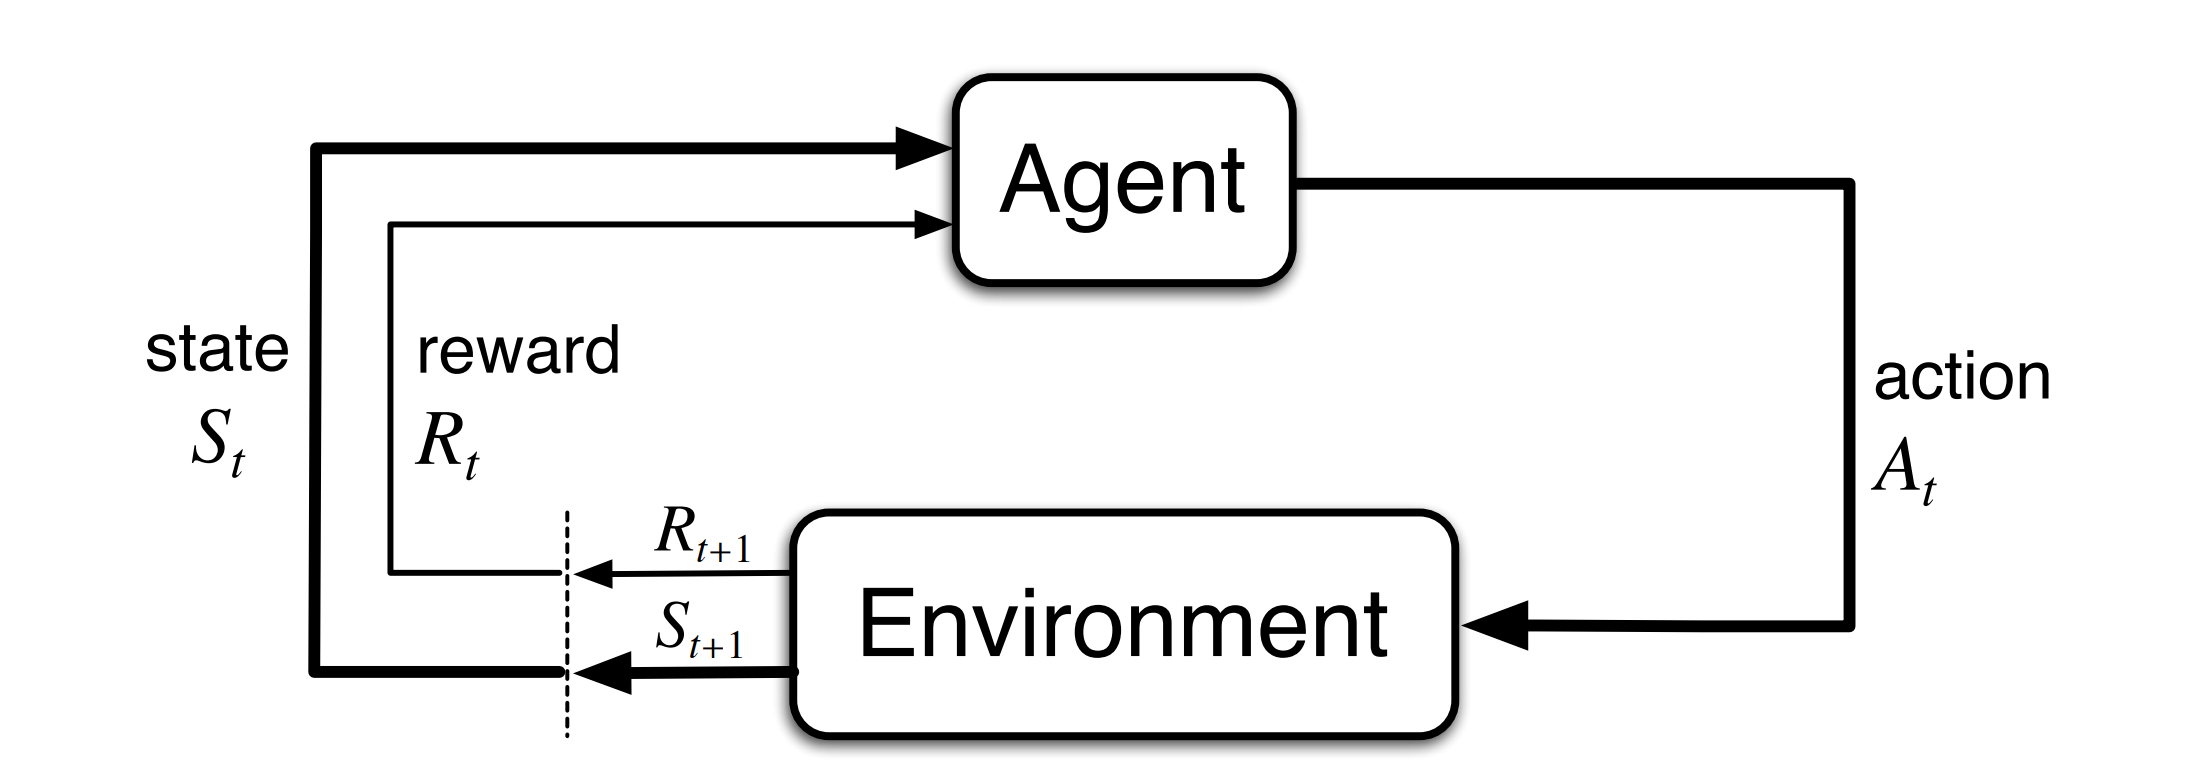
\includegraphics[width=\linewidth]{../img/agent_environment_interaction.png}
  \caption{Illustration of the agent environment interaction. Agent is in state $S_t$ and received reward $R_t$ for the last chosen action $A_{t-1}$, then $A_t$ is chosen by the agent and new state $S_{t+1}$ and reward $R_{t+1}$ are obtained. Image sourced from \cite[Figure 3.1.]{sutton2018reinforcement}.}
  \label{fig:agent_environment_interaction}
\end{figure}
\todo{should I write here explicitly that $S_t$, $A_t$ and $R_t$ are random variables?}

We now introduce the notion of a \textit{Markov decision process}, which is a formalisation of the agent environment interaction discussed above. The following is heavily inspired by \cite[Chapter 3]{sutton2018reinforcement}
\begin{defn}{Markov decision process}
\cite{sutton2018reinforcement}
\label{defn:markov_decision_process}

A Markov decision process is a 4-tuple $(\mathcal{S}, \mathcal{A}, \mathcal{P}, \mathcal{R}, \gamma)$, where 
\begin{enumerate}
\item $\mathcal{S}$ is the set of all possible states,
\item $\mathcal{A}$ is the set of all possible actions,
\item $\mathcal{P}(s_{t+1}|s_{t},a_t)=P(S_{t+1}=s_{t+1}|S_t=s_{t},A_t=a_t)$ is the probability that choosing action $a_t$ in state $s_t$ yields state $s_{t+1}$,
\item $\mathcal{R}(s_t, a_t)=R_{t+1}(S_t=s_t, A_t=a_t)$ is the reward received by choosing action $a_t$ in state $s_t$,
\item $\gamma \in [0,1)$ is the discount factor,

\end{enumerate}
\end{defn}
where $S_t$, $A_t$ and $R_t$ are random variables representing the state, action and reward at time $t$. The name Markov decision process is not a coincidence, notice that the state transition probabilities depend only on previous state and chosen action and not on the preceeding history. This means that the state must contain all information and no information is carried by the previously visited states and taken actions. Of course, this is a simplification and does not hold in real life (for example, the history of moves can hold information about the strength of a opponent in the game of chess), but it suffices to model even complex phenomena and allows for precise mathematical treatment. 

The agent chooses an action based on the current state to maximise the expected cumulative reward. A function that maps states to probabilities of actions is termed as \textit{policy}, see Definition \ref{defn:policy}.

\begin{defn}{Policy} \cite[Section 3.5]{sutton2018reinforcement}
\label{defn:policy}
Let $s \in \mathcal{S}$ and $a \in \mathcal{A}$. Then the policy is defined as
\begin{equation}
\pi(a|s)=P(A_t=a|S_t=s),
\end{equation}
where $P(A_t=a|S_t=s)$ is the conditional probability.
\end{defn} 

Another fundamental concept is the value function, see Definition \ref{defn:value_function}.

\begin{defn}{Value function} \cite[Section 3.5]{sutton2018reinforcement}
\label{defn:value_function}
Let $\pi$ be a policy and $s \in \mathcal{S}$. Then we define the value function $v_{\pi}(s)$ as
\begin{equation}
v_{\pi}(s)=\mathbb{E}_{\pi} \left[ \sum_{k=0}^{\infty} \gamma^k R_{t+k+1} | S_t=s \right],
\end{equation}
\end{defn}
where the subscript $\pi$ in $\mathbb{E}_{\pi}$ refers to the fact that the agent acts according to policy $\pi$.
The value function assigns each state the expected cumulative discounted reward -- the reward that the agent may expect to gain from state $s_t$ into the future. The discount factor $\gamma$ weights the future rewards by how far into the future they may be attained.

Another related notion is the \textit{action value function}, see Definition \ref{defn:action_value_function}.

\begin{defn}{Action value function} \cite[Section 3.5]{sutton2018reinforcement}
\label{defn:action_value_function}

Let $\pi$ be a policy and $s \in \mathcal{S}$ and $a \in \mathcal{A}$. Then we define the action value function $q_{\pi}(s,a)$ as
\begin{equation}
 q_{\pi}(s,a)=\mathbb{E}_{\pi} \left[ \sum_{k=0}^{\infty} \gamma^k R_{t+k+1} | S_t=s, A_t=a \right].
\end{equation}
\end{defn}
The action value function is much the same as value function, but it maps the actions taken in a state to the expected cumulative reward rather than just states. The action value function allows the agent to not always take the immediate most rewarding (greedy) action, but rather optimise the reward while taking into account the possible following states and actions. 

The value function and action value functions must be learned by exploring the environment. Unfortunately, the plethora of theory about estimation of these functions (e.g. using the Bellman equations) is out of scope of this thesis. We refer the interested reader to \cite[Section 3.5.]{sutton2018reinforcement} and the references therein. 

A slight twist on the definitions above is the \textit{advantage function}, see Defintion \ref{defn:advantage_function}.
\begin{defn}{Advantage function} \cite[Section 3]{a3c_paper}
\label{defn:advantage_function}

Let $\pi$ be a policy and $s \in \mathcal{S}$ and $a \in \mathcal{A}$. Denote the value function as $v_{\pi}(s)$ and the action value function as $q_{\pi}(s,a)$. Then we define the advantage function  as
\begin{equation}
 A_{\pi}(s,a) = q_{\pi}(s,a) - v_{\pi}(s).
\end{equation}
\end{defn}

Our aim is to obtain a policy that maximises the expected cumulative reward. We thus define the \textit{optimal policy}, \textit{optimal value function} and \textit{optimal action value function}, see Definition \ref{defn:optimal_definitions}.

\begin{defn}{Optimal policy, value function and action value function} \cite[Section 3.6]{sutton2018reinforcement}
\label{defn:optimal_definitions} \\
Let $R(\pi)$ be the expected cumulative reward obtained by following policy $\pi$. Then we define the optimal policy as
\begin{equation}
 	\pi^* = \underset{\pi}{argmax} \, R(\pi).
\end{equation}
Similarly, the optimal value function and optimal action value function are given by: 
\begin{equation}
 	v^*(s) = \underset{\pi}{\max} \, v_{\pi}(s)
\end{equation}
and
\begin{equation}
 	q^*(s,a) = \underset{\pi}{\max} \, q_{\pi}(s,a).
\end{equation}
respectively for $s \in \mathcal{S}$ and $a \in \mathcal{A}$.
\end{defn}
\todo{the definition of optimal policy is valid only for infinite horizon return!!! fix this}

\section{Exploration vs exploitation}
The optimal policy, value function and action value function must be learned by interacting with the environment. The agent now faces a dillema -- either to maximise his known reward (act greedily, but potentially get stuck in a local optimum) or explore the environment and update the policy in order to get the globally optimal policy. This exploration-exploitation tradeoff is always present with reinforcement learning and many approaches for dealing with it exist. An example are the $\epsilon$-greedy methods, where the agent acts greedily $1-\epsilon \, \%$ of the time and performs a random action $\epsilon \, \%$ of the time. $\epsilon$ is usually large at the beginning of training and decreased over time, the final threshold at which $\epsilon$ is kept constant is usually somewhere in $[0,0.1]$. For more information, we refer the reader to \cite[Section 2.7.]{sutton2018reinforcement}.

\section{Algorithm classes}
In this section, we to present a basic summary of current reinforcement learning methods with particular focus on policy-gradient methods.
\subsection{Model free vs. model based algorithms}
The most fundamental dividing line between reinforcement learning algorithms is whether the agent is given a model of the environment which allows the agent to take into account future states before they are experienced. The model is represented by the state transition function $\mathcal{P}$ as defined in Definition \ref{defn:markov_decision_process}. Having the model in hand obviously helps the agent learn tremendously, but having such a model in practice is quite rare, thus the model free methods are being used much more extensively. We focus on model free algorithms in this text.

\subsection{Model free methods}
In comparison to model based methods, the model free methods learn by trial and error.
Example of these methods are e.g. Monte Carlo Sampling, SARSA, Q-learning and Actor critic. These methods can be mainly divided into two groups -- value based methods and policy based methods. In this thesis, we focus particularly on the Actor critic method (as it will be used in the computational part of this thesis for reasons explained later), but we also give an introduction to Q learning, as it helps with understanding of how deep neural networks are used in the field of reinforcement learning (it is more complicated in the Actor critic case). We assume that the reader is familiar with basics of deep learning (such as architecture of neural networks and basic algorithms for training them such as stochastic gradient descent), a great introduction can be found in \cite[Part 2]{deep_learning_book}.
\subsubsection{Value based methods}
\subsubsection{$Q$ learning}
In this section, we follow \cite[Section 6.5.]{sutton2018reinforcement}.
The most famous example of a value based method is $Q$ learning.
Let $q^*(s,a)$ denote the optimal action value function as defined in Definition \ref{defn:optimal_definitions} and let $Q(s,a)$ be an estimate of $q^*(s,a), s \in \mathcal{S}, a \in \mathcal{A}$. If the sets $\mathcal{S}$ and $\mathcal{A}$ are finite, then the values of $Q(s,a)$ can be represented by a table and updated according to the updating rule presented in Equation \ref{eq:q_learning_updating_rule}.

\begin{equation}
Q(s_t, a_t) \leftarrow Q(s_t, a_t) + \alpha \left[r_{t+1} + \gamma \underset{a \in \mathcal{A}}{\max}Q(s_{t+1}, a) - Q(s_t, a_t) \right],
\label{eq:q_learning_updating_rule}
\end{equation}
where $\alpha$ is the learning rate, $\gamma$ is the discount factor, $s_t, a_t$ are the current state and current chosen action respectively, $s_{t+1}$ is the next state following action $a_t$, $r_{t+1}$ is the reward obtained by choosing action $a_t$ and the subscript $t$ is added to emphasize the transition between current and next step.
The whole algorithm can be summarised as follows:

\renewcommand{\algorithmicrequire}{\textbf{Input:}}
\renewcommand{\algorithmicensure}{\textbf{Output:}}


\begin{algorithm}
\small
\caption{Vanilla Q-learning \cite[p. 131]{sutton2018reinforcement}}\label{alg:q_learning}
\begin{algorithmic}
\Require{Choose the learning rate $\alpha \in (0,1]$ and exploration parameter $\epsilon>0$, number of episodes, initialise $Q(s, a), s \in \{s \, \mathrm{for} \,  s \, \mathrm{in} \, \mathcal{S} \, \mathrm{if} \, s \, \mathrm{is \, not \, final}\}$ and $Q(s,a)=0$ for $s$ final, $a \in \mathcal{A}$ (final state means that the environment is finished).}
\For{episode in $\{$1,...,number of episodes$\}$}
\State $s_t \leftarrow s_0$ Reset environment state 
\While{$s_t$ is not terminal}
\State $a_t \leftarrow$ Choose action a using an epsilon-greedy policy according to $Q(s_t,\cdot).$
\State $s_{t+1}, r_{t+1} \leftarrow$ act on action $a_t$, obtain new state $s_{t+1}$ and reward $r_{t+1} $
\State Update $Q(s_t,a_t)$ using Equation \ref{eq:q_learning_updating_rule}
\State $s_t \leftarrow s_{t+1}$
\EndWhile
\EndFor
\end{algorithmic}
\end{algorithm}
It has been shown that under the assumption that all state-action pairs continue to be updated during training, then $Q$ converges to $q^*$ almost surely \cite[p. 131]{sutton2018reinforcement}. This variant of $Q$-learning has an obvious problem -- it depends on a table for keeping the values of the $Q$ function and thus does not generalise to complex state spaces (such as infinite ones). To tackle this problem, a neural network has been introduced in place of the $Q(s,a)$ table as a function approximator, which we can then write as $Q(s,a;\theta)$, where $\theta$ are the weights of the neural network. This approach has been popularised by \cite{deep_q_learning_paper}, where they used $Q$-learning along with a neural network as a function approximator (and many other bells and whistles such as experience replay) to achieve superhuman performance on several Atari 2600 games. The reader interested in deep $Q$-learning can find the algorithm in \cite[Algorithm 1]{deep_q_learning_paper}.

\subsubsection{Policy approximation methods}
The theory of value based methods assumed that we estimate the value function and action value function and then based on them somehow choose the policy (such as taking the action with maximum value). However, another approach is possible -- modelling the policy explicitly. In this section, we mostly follow  \cite[Chapter 13]{sutton2018reinforcement}.

Policy approximation methods assume that the policy $\pi(a|s;\theta), a \in \mathcal{A}, s \in \mathcal{S}$ is dependent on parameters $\theta \in \R^d$ where $d \in \N.$ In general, the aim of these methods is to maximise some kind of performance measure $J(\theta)$. The performance measure $J$ is chosen such that the gradient $\nabla_{\theta}J$ exists and we can then write the very general updating rule as Equation \ref{eq:policy_approximation_updating_rule}.

\begin{equation}
\label{eq:policy_approximation_updating_rule}
\theta_{t+1}=\theta_t+\alpha \widehat{\nabla_{\theta_t} J(\theta_t)},
\end{equation}
where $\alpha$ is the learning rate and $\widehat{\nabla_{\theta_t} J(\theta_t)}$ is the estimate of the gradient of the performance measure $J$. Due to the aforementioned updating rule, these methods are also often called \textit{policy gradient methods}. 

\begin{rem} 
When using policy approximation methods, we do not need to randomly sample actions $\epsilon \%$ of the time to ensure exploration. All that is needed is to ensure that the policy does not become deterministic. This can be achieved by ensuring that $\pi(a|s;\theta) \in (0,1)$ \cite[Section 13.1]{sutton2018reinforcement}.
\end{rem}

A significant theoretical advantage compared to value based methods is that “~\textit{with continuous policy parameterization the action probabilities change smoothly as a function of the learned parameter, whereas in $\epsilon$-greedy selection the action probabilities may change dramatically for an arbitrarily small change in the estimated action values, if that change results in a different action having the maximal value. Largely because of this stronger convergence guarantees are available for policy-gradient methods than for action-value methods}” \cite[Section 13.2]{sutton2018reinforcement}. We refer the reader to the Policy gradient theorem located therein.

There exist also hybrid method between policy gradient methods and value based methods, where the policy, value function and action value function are all learned -- such methods are called \textit{actor critic} methods.

\subsubsection{Advantage actor critic}
In this section, we present the theory behind the (asynchronous) advantage actor critic (A3C) algorithm as developed in \cite{a3c_paper}.

The Advantage actor critic is a policy approximation algorithm that learns not only the policy but also the action value function. Let us first decipher the name of the algorithm. Advantage refers to the advantage function defined in Definition \ref{defn:advantage_function}, actor refers the learned policy approximation and critic refers to the learned action value function approximation (both the actor and the critic are neural networks that are used as function approximators). In practice, the actor and critic networks share some parameters (they can be thought of as a single neural net with diverging structure, such as a first shared layer and then diverging such that the second layer is not common to both the actor and the critic).

Denote the weights of the actor as $\theta$ and weights of the critic as $\theta_v$, thus the estimated policy can be written as $\pi(a|s;\theta)$ and the estimated value function as $v(s;\theta_v)$, $a \in \mathcal{A}, s \in \mathcal{S}$. The performance measure $J$ as mentioned in the previous section can be written as
\begin{equation}
J(\theta, \theta_v) = \nabla_{\theta'} \log \pi(a_t|s_t;\theta')A(s_t,a_t;\theta,\theta_v),
\end{equation}
\todo{check if J() is correct here, check if the definition of advantage function is correct}
where we again add the time subscript $t$ and where $\widehat{A}(s_t,a_t;\theta,\theta_v)$ is the advantage function given by 
\begin{equation}
\widehat{A}(s_t,a_t;\theta,\theta_v)=\sum_{i=0}^{k-1}\gamma^i r_{t+1} + \gamma^k V(s_{t+k};\theta_v) - V(s_{t};\theta_v),
\end{equation}
where $\gamma$ is the discount factor and where $k$ is the number of steps the agent has taken before the update, which is upper bounded by a chosen hyperparameter $t_{max}$. $t_max$ chooses at most how many steps the agent should take in an environment. The update is performed whenever a final state is reached or when $t_max$ steps have been taken.
\begin{rem}
Notice that in the formula for $\widehat{A}(s_t,a_t;\theta,\theta_v)$ the parameters $\theta$ are not explicitly present. In reality, the rewards $r_{(\cdot)}$ are chosen by the policy and thus depend on the parameters $\theta$. \todo{is this remark correct? please check} 
\end{rem}

The full A3C algorithm is given in \cite[Algorithm S3]{a3c_paper}. \todo{Should I write the full algorithm here? It would be exact copying of the algorithm from the paper, it is hard to write differently.} In the original paper, they made use of asynchronous updates to supposedly improve training stability. It was later shown in the paper \cite{a3c_asynchrony_not_necessary} that the asynchrony provides no added benefit in performance. Henceforth, when we refer to the Advantage actor critic, we mean the synchronous version and denote it shortly as A2C.